\documentclass[11pt]{article}
\usepackage[preprint]{acl_template/acl}
\usepackage{fontspec}
\setmainfont{Times New Roman}
\setsansfont{Arial}
\setmonofont{Menlo}[Scale=0.83]
\usepackage{microtype}
\usepackage{booktabs,graphicx,amsmath,array,float}
\usepackage{polyglossia}
\setdefaultlanguage{english}
\setotherlanguage{hebrew}
\newfontfamily\hebrewfont[Script=Hebrew]{Times New Roman}
\newcommand{\heb}[1]{\texthebrew{#1}}
\newcommand{\repo}[2]{\href{https://github.com/BenCarmel123/hebrew-acronym-disambiguation/blob/ef8c83d686895a32476acb28bfdb089947d050d5/#1}{#2}}

\title{Hebrew Acronym Expansion in Context:\\Free Generation and Candidate Selection}
\author{Ben Carmel \quad Shaked Schnarch \\
Tel Aviv University \\
\small NLP course project --- 14 October 2026}
\raggedbottom
\begin{document}
\maketitle
\begin{abstract}
Hebrew acronyms can have several meanings in context. Should a system generate an expansion freely or select from a supplied inventory, and how does a small task-trained Hebrew encoder compare with prompted language models? We study these questions on 381 test sentences, 77\% naturally occurring, comparing seven LLMs and two uses of DictaBERT. The inventory includes ordinary expansions and conventional interpretations such as gematria. Exact test acronym strings are absent from the documented train/dev files; historical training inputs and pretraining exposure are not fully known. In the main comparison, the task-trained encoder reaches 71.7\% in selection, competitive with local Qwen models (58.5--69.8\%), while API models score higher (83.2--93.7\%). Selection scores exceed generation scores for all six main LLMs. Candidate access and scoring differ together, so this gap does not isolate semantic ability. DictaLM is reported separately with an input-template limitation. The findings support candidate ranking as a practical local approach and show why answer format is central to evaluating acronym resolution.

\end{abstract}
\section{Introduction}
An acronym is a short written form that stands for a longer expression. In Hebrew, acronyms are written with a quotation mark before the last letter, as in \heb{ח״כ} (\heb{חבר כנסת}, ``member of parliament''), and they are common in news, parliamentary and everyday text. Many acronyms are ambiguous. For example, \heb{מט״ח} can mean \heb{מטבע חוץ} (foreign currency) or \heb{המרכז לטכנולוגיה חינוכית} (the educational technology center). Only the surrounding sentence tells the reader which one is meant.

\begin{figure*}[t]
\centering
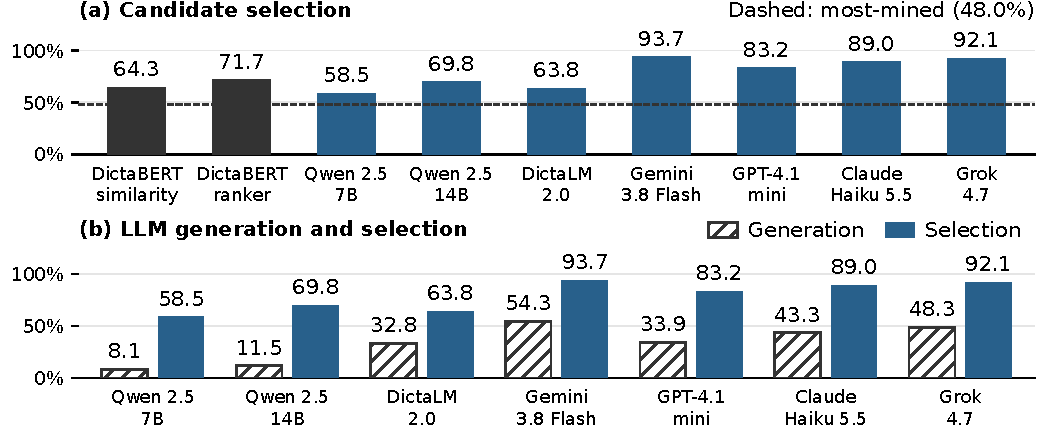
\includegraphics[width=\textwidth]{figures/generate_vs_select.pdf}
\caption{Automatic scores on 381 items, including failures. (a) Candidate selection across systems; encoders rank candidates without LLM text-label decoding. (b) The six LLMs in paired bars: generation uses \emph{normalized reference substring}, and selection uses \emph{strict label + reference match}. Candidate access and scoring rules differ, so the gap does not isolate model ability. Exact results: Table~\ref{tab:test-results}; DictaLM: Table~\ref{tab:dictalm-supplement}.}
\label{fig:generate-vs-select}
\end{figure*}

Hebrew adds challenges for matching an acronym to its dictionary entry. Prefixes such as ``in'', ``to'' and ``the'' attach directly to the word, so the acronym in a sentence may differ from its dictionary form. Earlier work addresses this problem by building Hebrew acronym dictionaries and using context to disambiguate their entries \citep{jacobs2020acronyms}. With language models, a further question arises: is the dictionary still useful when a model can generate an answer directly?

A language model can expand an acronym in two ways. In \emph{free generation}, it reads the sentence and writes the expansion. In \emph{candidate selection}, it is also given a list of possible expansions and picks one. Generation can produce an answer that is not on any list, but it can also produce a wrong or unsupported one. Selection limits the answer to the list, so it depends on the list being complete. We compare these two formats on the same occurrences. Our research question is how free generation and candidate selection compare under the tested conditions, and how a small task-trained Hebrew encoder compares with prompted language models. This matters when choosing between a local system built around an available dictionary and a general-purpose language model.

We run this comparison on a test set of 381 Hebrew sentences with label-review evidence that differs by source. Most (77\%) occur naturally, in parliamentary proceedings and on Wikipedia, and the rest were written by an LLM to add a second sense to types that had only one. We test three open LLMs, one of them the Hebrew-specialised DictaLM, four proprietary LLMs, and a pre-trained Hebrew encoder, used for pretrained similarity and task-trained candidate ranking. No exact test acronym string appears in the documented task-training or development files; the original training snapshot and pretraining exposure are not fully known. The task follows the stored inventory, including gematria and other conventional interpretations as well as ordinary expansions (Section~\ref{sec:data}).

Figure~\ref{fig:generate-vs-select} summarizes our findings. First, the task-trained encoder is competitive with the two local Qwen configurations at candidate selection, while the four API models score higher. Second, selection scores exceed generation scores for all six LLMs in the main comparison. This comparison changes both candidate access and the metric: strict candidate selection versus normalized reference-string inclusion. DictaLM appears in a separate supplementary table with a template caveat and four distinct measurements. These results motivate candidate ranking as a local option and make the answer space a central part of the system choice.

\section{Related Work}
\label{sec:related-work}
\paragraph{Hebrew acronyms.}
HAADS disambiguates abbreviations in Hebrew and Aramaic Jewish Law documents \citep{hacohenkerner2010haads}. \citet{jacobs2020acronyms} build an acronym dictionary for Modern Hebrew from unannotated text and use context to choose among its entries. Both treat the task as choosing from a dictionary and predate current LLMs. We study expansion in context with current models, and supply a candidate list only in the selection format.

\paragraph{Acronym disambiguation in English.}
SciAD formulates acronym disambiguation as choosing a long form from a dictionary-derived candidate set given the sentence and acronym \citep{veyseh2020acronym}. \citet{chen2023gladis} introduce GLADIS, an English benchmark with acronym-disjoint splits. Their model, AcroBERT, reads the context and one candidate together and learns to tell matching pairs from non-matching ones. Our encoder follows this pair-scoring idea but uses binary cross-entropy, whereas AcroBERT uses a triplet ranking objective. GLADIS builds many evaluation sentences by replacing full expressions with acronyms. We use mostly naturally occurring test sentences and keep substituted sentences for training.

\paragraph{Hebrew language models.}
DictaBERT is a BERT-style encoder pretrained on Hebrew text \citep{shmidman2023dictabert}, and DictaLM 2.0 is a Hebrew-adapted 7B LLM \citep{shmidman2024dictalm}. \citet{liang2026cognates} test 16 LLMs, including Qwen2.5-7B and DictaLM 2.0 Instruct, on Arabic--Hebrew word pairs with similar forms. Models lean on surface-form similarity, and DictaLM 2.0 Instruct scores near chance on both of their three-way tasks. All of their tasks are multiple choice, and they note that this may not reflect open-ended generation.

\paragraph{Answer format and scoring.}
Multiple-choice evaluation is convenient but sensitive to option order and identifiers \citep{zheng2024selection}, while open answers are hard to score automatically. \citet{agrawal2022large} ask GPT-3 to expand clinical abbreviations without choices, then map generated text to candidates by character overlap. \citet{meconi2025large} compare word-sense selection with generated definitions and explanations rated by an expert; strong free-form performance under that protocol shows why string agreement and semantic evaluation must be distinguished.

\paragraph{The gap.}
To our knowledge, no prior work compares free generation with candidate selection for Hebrew acronyms on the same occurrences, or compares a fine-tuned Hebrew encoder with current LLMs on this task. We do both, and measure how much the scoring rule changes generation results.

\section{Task and Data}
\label{sec:data}
\subsection{The unit of prediction}
Each item contains a sentence $x$, an acronym $a$, a candidate inventory $C$ and a reference answer $y\in C$. For the encoder, the target is marked in the sentence with \texttt{[ACR]} and \texttt{[/ACR]}; LLM prompts name the acronym alongside the original sentence (Section~\ref{sec:systems}).

Generation predicts an answer from sentence context and target information, without candidates. Selection picks one member of $C$ for the same item. We use \emph{expansion} as shorthand for the stored inventory answer: besides ordinary spelled-out expressions, it includes numerical interpretations in gematria (the use of Hebrew letters as numbers) and conventional or named uses that are not literal expansions. For example, the reference for \heb{ח״י} in one test sentence is \heb{שמונה עשרה בגימטריה} (eighteen in gematria; Table~\ref{app:res-examples}). Evaluation therefore measures agreement with this inventory and its reference labels, not only recovery of the words that formed an acronym.

The output spaces are:
\begin{equation}
\begin{aligned}
\hat{y}^{\mathrm{gen}}&=f(x,t)\in\Sigma^{*},\\
\hat{y}^{\mathrm{sel}}&=\operatorname*{arg\,max}_{c\in C}\mathrm{score}(x,t,c),
\end{aligned}
\end{equation}
where $t$ denotes the target information and $\Sigma^{*}$ is the set of text strings, so generation may return any string, while selection returns one candidate in $C$.

Table~\ref{tab:example} illustrates the interface with a constructed example, not a dataset item.
\begin{table}[t]
\centering\small
\begin{tabular}{@{}p{0.22\columnwidth}p{0.71\columnwidth}@{}}
\toprule
Sentence & \heb{ח״כ נשא נאום במליאה.} \\
Target & \heb{ח״כ} (the first token) \\
Generation & A short expansion, e.g.\ \heb{חבר כנסת} \\
Selection & A label assigned to one supplied candidate \\
\bottomrule
\end{tabular}
\caption{Illustrative input and answer formats. The sentence means ``A member of parliament gave a speech in the plenum.'' This is not a scored item.}
\label{tab:example}
\end{table}

\subsection{Sources and construction}
The candidate inventory lists 2,702 possible expansions for 638 acronym types. Of these, 2,002 come from Hebrew Wikipedia and Wiktionary abbreviation pages, 636 are gematria readings, and 64 were added by hand when a reviewer found a missing sense while checking Knesset sentences, some of them test sentences. The inventory is therefore not a dictionary built independently of the test set. Sentences come from Hebrew Wikipedia and from the Knesset Corpus, a collection of Israeli parliament plenary transcripts released by the University of Haifa (\texttt{HaifaCLGroup/KnessetCorpus} on Hugging Face). Mining kept sentences of 40--200 characters with a clear acronym boundary (allowing attached prefixes) and no definitions or other acronyms; a few retained items still break these rules.

\subsection{Train, development and test sets}
Table~\ref{tab:data} gives the size of the documented files and their kinds of sentence. \emph{Natural} sentences contain the acronym as written. \emph{Substituted} sentences come from Wikipedia: a spelled-out expansion was replaced with the acronym, and the removed expression serves as a weak label. \emph{Deglossed} sentences are natural sentences with an adjacent explanation removed. \emph{Claude-authored} sentences were written by an LLM to add senses to types that had few. Substituted and authored sentences give labels cheaply, but need not read like naturally abbreviated text.

\begin{table}[t]
\centering\small
\begin{tabular}{@{}lrrr@{}}
\toprule
Quantity & Train & Dev & Test \\
\midrule
Items & 2,829 & 62 & 381 \\
Acronym types & 434 & 11 & 60 \\
\midrule
Substituted Wikipedia & 2,316 & 0 & 0 \\
Natural Knesset & 319 & 62 & 253 \\
Natural Wikipedia & 50 & 0 & 41 \\
Deglossed Wikipedia & 8 & 0 & 0 \\
Claude-authored & 136 & 0 & 87 \\
\bottomrule
\end{tabular}
\caption{Items by set and by kind of sentence. Every item has at least two candidates.}
\label{tab:data}
\end{table}

\paragraph{Train.} The documented encoder training file contains 2,829 items, which give 12,684 sentence--candidate pairs. Most labels are weak labels from substitution, reused without reannotation. Regenerating the preparation reproduces 2,665 of these rows; the other 164 are 136 authored examples and 28 truncated contexts.

\paragraph{Development.} The documented development set holds 62 natural Knesset items for 11 types. The training code selects by development loss; the selected historical epoch is unrecorded. Its labels combine reused human reviews and AI-assisted author decisions. Each of its types has a single observed sense.

\paragraph{Test.} The test set has 381 items for 60 acronym types: 253 Knesset, 41 Wikipedia and 87 Claude-authored sentences. Their labels have different review records. A human reviewed all 253 Knesset labels, confirming 221 and correcting 32; the original labels of the corrected items were not kept. The 87 authored items, three sentences for each of 29 types, are marked as human-reviewed. The 41 Wikipedia items are marked as verified, but no review verdict was recorded. One person reviewed the labels, so no inter-annotator agreement is available. We removed 14 Knesset items from four protocols that also supply training items, leaving 381 of the original 395; all scores use these 381, although some saved runs also hold responses for the removed items. This label review is separate from the review of model responses in Section~\ref{sec:eval}.

\subsection{Separation of the sets}
\label{sec:separation}
We split by acronym type. Exact acronym and sentence strings are disjoint across the train, development and test files, and the test set shares no document with train or development. Train and development share three documents. Near-identical forms can still cross the split: the final-letter variants \heb{אג״ם}/\heb{אג״מ} and \heb{מל״ם}/\heb{מל״מ} affect seven test items, and prefixed forms can cross it too. The split therefore tests unseen acronym strings, not unseen acronym families.

\section{Systems and Experimental Design}
\label{sec:systems}
The encoder ranks candidates; each LLM performs both generation and selection. Only the ranker receives task-specific supervised training. All LLMs get the same prompt for each task, and selection shows the candidates in the same seeded, shuffled order for every item. These controls align inputs but do not make the systems equivalent. The models also differ greatly in size: DictaBERT has about 0.2B parameters (184 million in the saved reconstruction), compared with 7B and 14B for Qwen. Parameter counts for the four proprietary models are not available in the saved records.

\subsection{Supervised Hebrew candidate ranker}
DictaBERT is a pretrained Hebrew encoder \citep{shmidman2023dictabert}. Our implementation is a \emph{cross-encoder}: the marked sentence and one candidate are encoded jointly, so their tokens can attend to each other. A dropout layer and a linear head turn the pooled representation into a scalar score. Candidates are scored independently, and prediction chooses the highest score within the item's candidates.

For each training item, the reference candidate is positive and the other candidates are negative. The objective is binary cross-entropy on the pair scores, over $M$ sentence--candidate pairs:
\begin{equation}
\mathcal{L}=-\frac{1}{M}\sum_{j=1}^{M}\big[z_j\log p_j+(1-z_j)\log(1-p_j)\big].
\end{equation}
Here $p_j=\sigma(u_j)$ is the sigmoid of pair score $u_j$, and $z_j$ is 1 for the reference candidate and 0 otherwise. AdamW updates the whole model, with no adapter.

The reference Colab notebook specifies dropout 0.1, learning rate $2\times10^{-5}$, pair batch size 16, one epoch and checkpoint selection by lowest development pair loss. The authors attribute the supplied weights to Ben's Colab run based on \texttt{dicta-il/dictabert}. The historical training manifest is incomplete: the executed seed, exact input snapshot and selected epoch/loss are unknown. These are documented settings, not a reproduced training run; the checkpoint documentation records the available evidence (Section~\ref{sec:artifacts}).

The saved inference reconstruction verifies the full state dictionary, including its scoring head. Each pair is the marked sentence followed by the candidate, joined by BERT special tokens. Context is cropped from the outside toward a nominal 256-token limit while retaining the target and candidate. Required tokens can exceed that limit in the historical Colab encoder. Test spans use the recorded first quote-normalized occurrence, with attached letters outside the marked span; these are automatic spans, not human annotations. The LLMs receive the full original sentence.

The similarity baseline also uses pretrained DictaBERT, without task adaptation. Its implementation encodes the marked context and each candidate separately and chooses the highest cosine similarity between their \texttt{[CLS]} vectors. The cross-encoder instead jointly represents each pair and uses a learned scoring head. Their comparison therefore changes input representation and decision rule as well as training. The similarity predictions are preserved, but their original run manifest and sentence snapshot are unavailable.

\subsection{Prompted language models}
The generation prompt, written in Hebrew, gives the original sentence and names the acronym separately, asking for its expansion in a few words without explanation. It supplies neither candidates nor the reference. The selection prompt adds the candidate list and requests one label, such as A or AA, with no extra text. Neither prompt includes worked examples; the selection inventory does contain the reference. We use \texttt{qwen2.5:7b} and \texttt{qwen2.5:14b} \citep{qwen2025technical} through Ollama with Q4\_K\_M quantization, the Hebrew-specialised DictaLM 2.0 Instruct \citep{shmidman2024dictalm} (7.25B parameters, \texttt{dictalm2.0-instruct-GGUF}, Q4\_K\_M) through Ollama with temperature 0 and seed 42,
\texttt{gemini-3.8-flash} with low thinking, \texttt{gpt-4.1-mini-2025-04-14}, \texttt{claude-haiku-5-5}, and \texttt{grok-4.7} with low reasoning and no tools. Each item has one scored response per task; collection logs retain technical attempts. The saved Qwen 7B settings explicitly record temperature 0, seed 42 and \texttt{num\_predict=512}; Qwen 14B records the same options. These settings do not establish full determinism, and low thinking is not disabled thinking. Full prompts, response identities and run settings are preserved in the saved-result exports.

\section{Evaluation}
\label{sec:eval}
\subsection{Scoring}
All reported test scores retain the same 381 items, including failures. For candidate selection, the chosen candidate must equal the reference expansion. An LLM response must contain exactly one in-range uppercase label after trimming boundary whitespace. Labels are A--Z, AA, AB, and so on; two items have 30 candidates. A response such as ``A.'' or a label followed by candidate text is invalid under this strict rule.

For generation, the automatic rule checks whether the reference expansion occurs as a substring after quote normalization, with boundary whitespace stripped from the reference. It can accept a longer answer containing the reference and reject a valid variant, such as \heb{שקלים חדשים} for \heb{שקל חדש}. Thus generation measures reference-string inclusion, whereas selection measures strict label decoding followed by candidate equality. The two percentages are not the same measure of semantic correctness. For either rule we report
\begin{equation}
\mathrm{Score}=\frac{1}{N}\sum_{i=1}^{N}c_i,
\end{equation}
where $c_i=1$ when the response passes the relevant rule and $N=381$. Technical failures, including truncated responses, score zero.

Technical completion, stored format validity and automatic matching are separate fields. For generation, the stored validity flag means that \emph{any} candidate occurs in the response under normalization; it is not a general test of well-formed output. Qwen 14B generation, for example, has 10/381 technical failures (2.6\%), which remain in the denominator. Per-arm completion and validity counts are supplied with the results (Section~\ref{sec:artifacts}).

\subsection{Human review and the DictaLM diagnostic}
The closed review export covers 741 of 4,953 responses from the six main LLMs and the trained encoder. A single annotator (S.S.) saw system identity, with a negative default and selective coverage of about 24--79\% of technically complete generation negatives across the six LLMs. Here \texttt{fits} meant agreement with the displayed reference, not independent contextual correctness; review against an erroneous reference cannot validate it. S.S. retrospectively clarified that he had not seen AI evaluations of the answers before annotating; the historical exposure field remains unknown. Nine unresolved response judgments concern four items, six sharing a grouped decision, not nine independently adjudicated gold errors. Batch timestamps do not measure per-item reading time. This review diagnoses disagreements but supports neither population accuracy nor cross-system human rankings.

Author annotation (B.C.) provides a separate, complete layer for DictaLM's 381 generated responses. The consolidated review table preserves 193 accepted responses; the acceptance rule is only partly documented, and blinding is not documented. We report this acceptance rate without reconstructing a richer rule or applying it to other models.

DictaLM selection is also reported with a diagnostic parser that reads a leading label from an otherwise invalid response. This does not replace strict scoring. In addition, its saved chat template lacks the newline after \texttt{[/INST]} specified by the publisher's \href{https://huggingface.co/dicta-il/dictalm2.0-instruct-GGUF\#instruction-format}{GGUF instruction format}. The tokenized request was not logged and the effect of this mismatch is unknown. We therefore present all four DictaLM measurements in a separate supplementary table, without a common ranking.

\subsection{Reference points and variability}
We report four reference points: random choice among the candidates; the candidate with the most Wikipedia hits (most frequent); the candidate that yielded the most mined sentences (most mined); and an oracle that is right whenever the reference is among the candidates. The recorded most-mined score, 183/381 (48.0\%), is an optimistic, non-held-out reference influenced by test-containing mining counts. A direct equality check links counts to Wikipedia source totals for pairs covering 32/41 Wikipedia test items; the original count producer is absent, so inclusion of all 41 is not established. Count-subtraction diagnostics are not recovered leakage-free baselines. Candidate order is shuffled with seed 42 and preserved per item. Each system has one reported run, one prompt per task and one candidate order per item, without variability estimates. Option order and identifiers can affect LLM choices \citep{zheng2024selection}, which this design does not test. Items from the same type or document are not independent. The identified exports retain per-response rules and run IDs; the main notebook documents the saved-result analysis without requiring model execution.

\subsection{Reproducibility artifacts}
\label{sec:artifacts}
The \repo{notebooks/experimental_study.ipynb}{analysis notebook} and \repo{saved-results/README.md}{saved-evidence guide} link to published revision \texttt{4d2dc73}. Later documentation and DictaLM annotation supplements are in the accompanying local snapshot, not yet published. The notebook reads hash-identified saved responses without model requests or weights. \path{results/submission-20261010/README.md} maps tables to predictions, review bindings, prompts and settings; \path{docs/checkpoints.md} records inference reconstruction and historical training gaps. This reproduces saved-result analysis, not training or hosted-model responses.

\section{Results and Discussion}
\label{sec:results}
Figure~\ref{fig:generate-vs-select} and Table~\ref{tab:test-results} give the main comparison. Two results stand out: the trained encoder scores above all three local LLMs at selection, with a small lead over Qwen 14B, and selection scores higher than generation for every LLM under the automatic rules.
\begin{table}[H]
\centering\small
\begin{tabular}{@{}lrr@{}}
\toprule
System & Generation & Selection \\
\midrule
Random & -- & 23.5 \\
Most frequent & -- & 37.0 \\
Most mined & -- & 48.0 \\
Oracle & -- & 100.0 \\
\midrule
DictaBERT similarity & -- & 64.3 \\
DictaBERT ranker & -- & 71.7 \\
\midrule
Qwen 2.5 7B & 8.1 & 58.5 \\
Qwen 2.5 14B & 11.5 & 69.8 \\
DictaLM 2.0 & 32.8 & 63.8 \\
Gemini & 54.3 & 93.7 \\
GPT-4.1 mini & 33.9 & 83.2 \\
Claude Haiku 5.5 & 43.3 & 89.0 \\
Grok 4.7 & 48.3 & 92.1 \\
\bottomrule
\end{tabular}
\caption{Test scores (\%) on 381 items, failures counted as wrong. Generation: reference substring. Selection: exact candidate, using the same post-hoc leading-label rule for all seven LLMs. Similarity uses pretrained DictaBERT. The ranker is task-trained. Most mined is optimistic (Section~\ref{sec:eval}).}
\label{tab:test-results}
\end{table}

\subsection{The task-trained encoder}
\label{sec:res-encoder}
The trained encoder selects the reference in 273 of 381 items (71.7\%). It beats Qwen 7B by 13.1 points and the Hebrew-specialised DictaLM 2.0 by a small margin of 7.9 points (273 versus 243 items), and trails the weakest API model, GPT-4.1 mini, by 11.5 points. Against Qwen 14B the encoder leads by seven items (1.8 points) with only about 1.2\% of its parameters (184M versus 14.8B, roughly 80 times fewer), although the margin is small, and correcting three known reference errors (Section~\ref{sec:limitations}) gives 274 versus 269. Compared with the pretrained similarity baseline's 245 correct items (64.3\%), the trained ranker adds 28 (7.3 points), although the two also differ in architecture. Like AcroBERT \citep{chen2023gladis}, the ranker scores context--candidate pairs, so it can rank candidates for acronyms it never saw in training.

\subsection{Generation versus selection}
\label{sec:res-formats}
Selection scores exceed generation scores for each of the seven LLMs (Figure~\ref{fig:generate-vs-select}b), by 31.0 points for DictaLM to 58.3 points for Qwen 14B. The two formats differ in more than candidate access: generation is checked by string inclusion, while selection must return a valid label, and the inventory contains every test reference (100\% oracle coverage), partly through review-time additions. The gap therefore does not isolate the effect of seeing candidates.

Reference wording explains part of the gap. In 67 of the 381 items the reference contains parentheses, such as \heb{שמונה עשרה (גימטריה)} (eighteen, gematria) for \heb{י״ח} in \texttt{kn4-0499}. Across the seven LLMs, these items yield 1 of 469 automatic generation matches against 366 of 469 selection matches. Grok's \heb{שמונה עשר (18)} is rejected by the string rule but judged to fit by the reviewer. On the remaining 314 items selection still leads for all seven systems (Gemini: 207 versus 294 matches). The selective review also marks 338 automatically rejected generated answers as agreeing in meaning with the displayed reference, so the generation scores are likely underestimates. A common semantic assessment of both formats is needed to compare answer correctness.

\subsection{Results by kind of sentence}
\label{sec:res-source}
The trained encoder's gain over the similarity baseline comes from Knesset items (146 to 177 of 253), while the two are close on Wikipedia (31 to 30 of 41) and authored items (68 to 66 of 87) (Table~\ref{tab:res-source}). Against Qwen 14B, the encoder leads on Knesset items (177 versus 166) and trails slightly on Wikipedia (30 versus 32) and authored items (66 versus 68). The sources also differ in acronym mix, so these differences are not effects of source alone.

\begin{table}[t]
\centering\small
\setlength{\tabcolsep}{3pt}
\begin{tabular}{@{}lrrr@{}}
\toprule
System & Knesset & Wikipedia & Authored \\
\midrule
DictaBERT similarity & 57.7 & 75.6 & 78.2 \\
DictaBERT ranker & 70.0 & 73.2 & 75.9 \\
\midrule
Qwen 7B, gen. & 8.7 & 12.2 & 4.6 \\
Qwen 7B, sel. & 54.5 & 70.7 & 64.4 \\
Qwen 14B, gen. & 13.0 & 17.1 & 4.6 \\
Qwen 14B, sel. & 65.6 & 78.0 & 78.2 \\
DictaLM 2.0, gen. & 33.2 & 48.8 & 24.1 \\
DictaLM 2.0, sel. & 64.4 & 75.6 & 56.3 \\
Gemini, gen. & 47.8 & 78.0 & 62.1 \\
Gemini, sel. & 94.9 & 95.1 & 89.7 \\
GPT-4.1 mini, gen. & 32.8 & 51.2 & 28.7 \\
GPT-4.1 mini, sel. & 83.0 & 90.2 & 80.5 \\
Claude Haiku, gen. & 39.5 & 73.2 & 40.2 \\
Claude Haiku, sel. & 89.7 & 92.7 & 85.1 \\
Grok, gen. & 44.3 & 68.3 & 50.6 \\
Grok, sel. & 94.1 & 95.1 & 85.1 \\
\bottomrule
\end{tabular}
\caption{Test scores (\%) by source (253, 41 and 87 items), with the rules of Table~\ref{tab:test-results}.}
\label{tab:res-source}
\end{table}

\subsection{Hebrew specialisation and hand judgment}
\label{sec:res-measurement}
DictaLM 2.0 and Qwen 7B have similar sizes (7.25B and 7.6B) and run with the same local inference settings. DictaLM generates the reference four times as often (32.8\% versus 8.1\%) but gains only 5.3 points in selection (63.8\% versus 58.5\%). Hebrew-specialised training is one possible explanation, but base-model and chat-template differences prevent attributing the gap to specialisation. To see how much the generation rule matters, B.C. judged all 381 DictaLM generated answers by hand (Table~\ref{tab:dictalm-supplement}). The automatic rule accepts 125 answers and B.C. 193, with 121 accepted by both, 72 only by hand and four only automatically.

\begin{table}[H]
\centering\small
\begin{tabular}{@{}lrr@{}}
\toprule
DictaLM measurement & Count & \% \\
\midrule
Generation: automatic & 125/381 & 32.8 \\
Generation: by hand (B.C.) & 193/381 & 50.7 \\
Selection: bare label only & 0/381 & 0.0 \\
Selection: leading label & 243/381 & 63.8 \\
\bottomrule
\end{tabular}
\caption{DictaLM 2.0 under different scoring rules (381 items). Main results use the automatic generation and leading-label selection rows, the rules applied to every LLM.}
\label{tab:dictalm-supplement}
\end{table}

\subsection{Examples and errors}
\label{sec:res-errors}
Table~\ref{app:res-examples} in Appendix~\ref{app:tables} shows a correct generated answer that the string rule rejects, a selection answer with extra text after the label, and an encoder error. Appendix~\ref{app:examples} gives more examples, and Appendix~\ref{app:prompts} gives both prompts.

\subsection{Conclusions}
\label{sec:conclusions}
We draw two conclusions.

\emph{A small task-trained encoder is competitive with local LLMs when a candidate list exists.} DictaBERT, with 184M parameters, reaches 71.7\% in selection. It beats Qwen 7B and the Hebrew-specialised DictaLM 2.0, a 7.25B LLM, and scores close to Qwen 14B with about 1.2\% of its parameters. The margins over Qwen 14B and DictaLM are small for a single run, and the four API models remain ahead (83.2--93.7\%). In practice, when a Hebrew acronym inventory is available, a small trained ranker is a strong alternative to a local LLM.

\emph{Choosing from candidates scores higher than writing the expansion freely.} Selection scores higher than generation for all seven LLMs under the automatic rules, by 31.0 to 58.3 points. Part of this gap comes from the different scoring rules and reference wording: judged by hand, DictaLM's generation rises from 32.8\% to 50.7\%, and the selective review marks 338 automatically rejected answers of the other models as agreeing with the displayed reference. Future evaluations should judge both formats by the same semantic criterion. When an inventory covers the intended senses, selection is a practical choice supported by these higher automatic scores. Generation remains necessary for acronyms or senses missing from the list, and string matching misses valid variants.

\subsection{Future work}
\label{sec:future}
\paragraph{More and cleaner training data.} The documented training file has 2,829 items, most of them weakly labeled substituted sentences. Its identity as the historical run input remains unverified. Mining more natural sentences and cleaning their labels would show how far task training can take a small encoder, and whether its gap to the API models narrows. Our sentences come from only two sources, Wikipedia and parliamentary transcripts. Other kinds of Hebrew text could add senses that our sources rarely use: news, legal rulings, medical and military writing, informal social-media posts, and Rabbinic literature, the domain of HAADS \citep{hacohenkerner2010haads}. Mining them would test whether the encoder generalizes beyond our two sources.

\paragraph{Training the LLMs too.} We compare a fine-tuned encoder with LLMs used without task training, so training and model type change together. Fine-tuning an open LLM such as DictaLM 2.0 on the same training data, for example with a parameter-efficient method, would separate the effect of task training from that of architecture and size.

\paragraph{A common semantic score.} Generation and selection are now scored by different rules. Judging every answer of every model by the same semantic criterion, with two annotators and an agreement estimate, would measure the true gap between the formats. An LLM judge could reduce this effort if it is first validated against those human labels.

\paragraph{Variability and robustness.} Each system ran once. Training the encoder with several seeds set before initialization, and running the LLMs with several candidate orders and prompt wordings, would show how stable the differences are.

\paragraph{Harder and cleaner tests.} Newly coined acronym--meaning pairs in informative contexts would separate contextual interpretation from familiar associations. Varying candidate-set size, hard distractors and option order would test how selection depends on the list. Since chance is $1/k$ for $k$ candidates, such a test must control for chance. Finally, independently validating the test references would remove known errors, such as the three wrong labels in Section~\ref{sec:limitations}.

\section{Limitations}
\paragraph{Data and labels.} The test set mixes natural and authored text, with different label-review evidence by source (Section~\ref{sec:data}). Domain, construction and acronym mix differ from the mostly substituted training data. The small development set also has label defects: one \heb{מט״ח} sentence about the educational technology center is labeled foreign currency, limiting checkpoint selection and development comparisons. Named uses follow local conventions: development accepts \heb{רבי משה בן מימון} for \heb{רמב״ם} even in hospital and street contexts. A stored reference is therefore not a complete account of valid interpretations. Separation claims remain limited to the documented files (Section~\ref{sec:separation}).

\paragraph{Measurement and comparison.} The scoring and review limits in Section~\ref{sec:eval} preclude a common semantic ranking; DictaLM also has a template mismatch. Models differ in supervision, architecture and size, and the single-run design does not estimate variability. Incomplete historical training records and similarity-run provenance further limit reproducibility. Broader claims require evaluation beyond these model configurations and a common semantic assessment of generated and selected answers.

\label{bodyend}
\bibliography{references}
\clearpage
\appendix
\section{Additional result tables}
\label{app:tables}
Table~\ref{app:res-examples} shows two saved responses discussed in Section~\ref{sec:res-errors}.

\begin{table}[!htbp]
\centering\small
\begin{tabular}{@{}p{0.24\columnwidth}p{0.68\columnwidth}@{}}
\toprule
Item / system & Saved evidence \\
\midrule
\texttt{kn-0002}\newline DictaLM &
Context excerpt: \heb{עודף של 650 מיליון ש"ח.}\newline
Reference: \heb{שקל חדש} (new shekel).\newline
Generation: \heb{ש"ח = שקלים חדשים.}\newline
Automatic: no; author (B.C.): yes.\newline
Selection: \texttt{C.} \heb{שקל חדש}, read as C: correct. \\
\midrule
\texttt{kn4-0048}\newline DictaBERT ranker &
Context excerpt: \heb{18 תומכים, ח"י תומכים}\newline
Reference: \heb{שמונה עשרה בגימטריה} (eighteen in gematria).\newline
Selected: \heb{חוק יסוד} (Basic Law).\newline
Exact candidate match: no. \\
\bottomrule
\end{tabular}
\caption{Two Knesset test items with saved responses (Section~\ref{sec:artifacts}).}
\label{app:res-examples}
\end{table}

\section{Prompts}
\label{app:prompts}
Every LLM received the same prompt text (Section~\ref{sec:systems}). Below are both prompts for test item \texttt{kn-0002}, with our English translation. The selection prompt lists the candidates in the item's fixed shuffled order.

\paragraph{Generation.}
\heb{בהתחשב במשפט הבא בעברית, מהו הפירוש של ראשי התיבות "ש״ח"?}\\
\heb{ענה במילים ספורות בלבד, ללא הסבר.}\\
\heb{משפט: ומשום שהעולים לא מגיעים נוצר בתקציב משרד הקליטה עודף של 650 מיליון ש"ח.}\\
\heb{פירוש:}

\noindent\emph{Translation:} ``Given the following Hebrew sentence, what is the meaning of the acronym `\heb{ש״ח}'? Answer in a few words only, without explanation. Sentence: \ldots{} Meaning:''

\paragraph{Selection.}
\heb{בהתחשב במשפט הבא בעברית, מהו הפירוש של ראשי התיבות "ש״ח"?}\\
\heb{ענה בסימון של אפשרות אחת בלבד (למשל: \LR{A} או \LR{AA}), בלי שום טקסט נוסף.}\\
(the sentence line, as above)\\
A. \heb{ש.ח.} \quad B. \heb{שטר חוב} \quad C. \heb{שקל חדש}\\
D. \heb{שידור חוזר} \quad E. \heb{שלוש מאות ושמונה (גימטריה)}\\
F. \heb{שומר חינם}\\
\heb{תשובה:}

\noindent\emph{Translation of the second line:} ``Answer with the label of one option only (for example: A or AA), without any additional text.'' The last line means ``Answer:''.

\section{Test label distribution}
\label{app:labels}
Test items have between 2 and 30 candidates (median 4, mean 5.0); seven items have two candidates and two items have 30. Of the 60 acronym types, 22 have a single reference sense in the test set, 37 have two and one has three. The most common test sense of each type covers 306 of the 381 items (80.3\%). This share is computed from test labels, so it describes the label distribution and is not a baseline.

\section{Further examples}
\label{app:examples}
Table~\ref{app:examples-table} adds four saved responses: a correct answer rejected by the string rule, two clear generation errors, and an item with a known wrong reference (Section~\ref{sec:limitations}).

\begin{table}[!htbp]
\centering\small
\begin{tabular}{@{}p{0.24\columnwidth}p{0.68\columnwidth}@{}}
\toprule
Item / system & Saved evidence \\
\midrule
\texttt{kn4-0499}\newline Grok, gen. &
Context excerpt: \heb{מחר, יום רביעי, י"ח בחודש טבת}\newline
Reference: \heb{שמונה עשרה (גימטריה)} (eighteen, gematria).\newline
Generation: \heb{שמונה עשר (18)}.\newline
Automatic: no; human review: fits. \\
\midrule
\texttt{kn-0022}\newline Qwen 7B, gen. &
Context excerpt: \heb{בעלות ממוצעת של כ-42 ש"ח לצו}\newline
Reference: \heb{שקל חדש} (new shekel).\newline
Generation: \heb{שטרות חשמל} (electricity bills).\newline
Automatic: no; human review: does not fit. \\
\midrule
\texttt{kn4-0554}\newline Qwen 7B, gen. &
Context excerpt: \heb{טקס ההשבעה של ארגון "אי"ל"}\newline
Reference: \heb{ארגון יהודי לוחם} (fighting Jewish organization).\newline
Generation: \heb{ארגון איסלאמי} (Islamic organization).\newline
Automatic: no; human review: does not fit. \\
\midrule
\texttt{kn4-0207}\newline Gemini, sel. &
Context excerpt: \heb{מסכת בבא מציעא, דף ס"ב}\newline
Reference: \heb{סודי ביותר} (top secret), a known wrong label.\newline
Selected: \heb{שישים ושתיים (גימטריה)} (sixty-two, gematria), the page number.\newline
Automatic: no. \\
\bottomrule
\end{tabular}
\caption{Further saved responses. Human review refers to the selective review of Section~\ref{sec:eval}.}
\label{app:examples-table}
\end{table}

\clearpage
\section*{AI Disclosure and Reflection}
While preparing the proposal, we used AI tools to find data sources, review relevant papers, and run preliminary robustness checks. This helped us narrow the research question and explore promising directions. These early checks are separate from the experiments reported here.

During data preparation, AI tools helped us write web-scraping code. Claude generated sentences for underrepresented acronym senses: the documented dataset includes 136 such training examples and 87 test examples, reported separately from natural text. AI assistance also supported some author decisions about labels. Section~\ref{sec:data} describes label provenance and human-review coverage. AI assessments of model responses are kept separate from human judgments.

OpenAI Codex also helped with implementation, literature checking, and drafting and revising the report. We found the tools useful for exploring options and working through technical problems, but their suggestions needed checking. Plausible labels were not always appropriate in context, and convincing explanations did not always match the evidence. Checking sources, examples, and saved results was therefore an important part of the work.

\end{document}
